%!TEX root = ../thesis.tex
% ******************************* Thesis Appendix A ****************************

\chapter{}
\section{N-1 plots for cut-scan results}\label{app:n-1_plots_cut_opt}

\ifpdf
\graphicspath{{chapter-optimisation/Figs/Raster/}{chapter-electroweak/Figs/PDF/}{chapter-optimisation/Figs/}}
\else
\graphicspath{{chapter-optimisation/Figs/Vector/}{chapter-electroweak/Figs/}}
\fi

\begin{figure}
	\centering
	\begin{subfigure}[b]{0.5\linewidth}
		\centering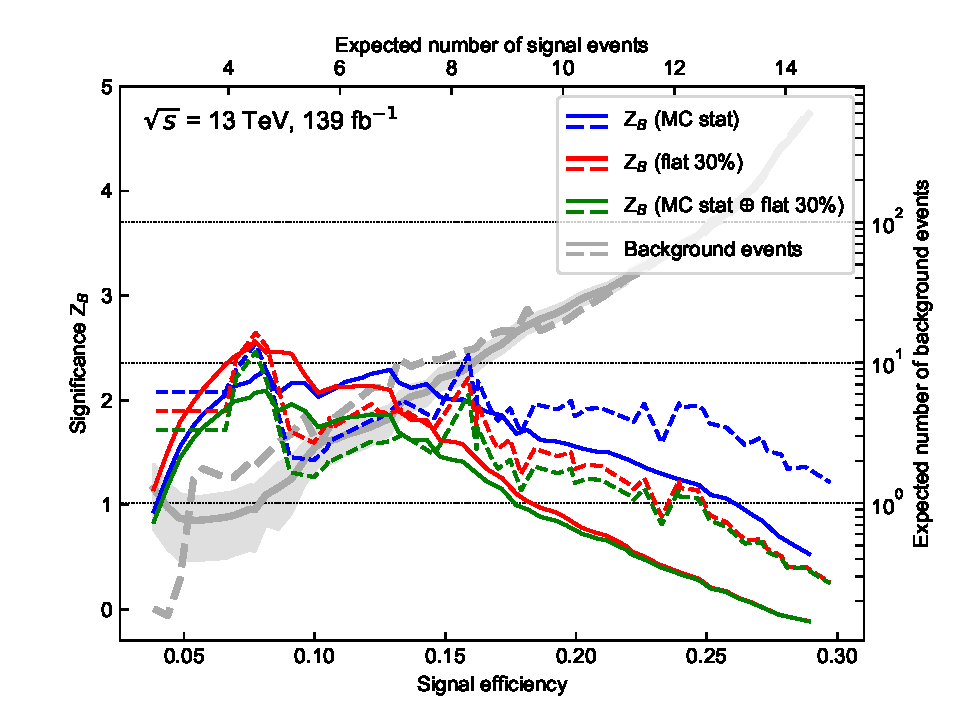
\includegraphics[width=1.0\textwidth]{N-1_cut_scan/z_vs_effs_800_150.pdf}
		\caption{}
	\end{subfigure}\hfill
	\begin{subfigure}[b]{0.5\linewidth}
		\centering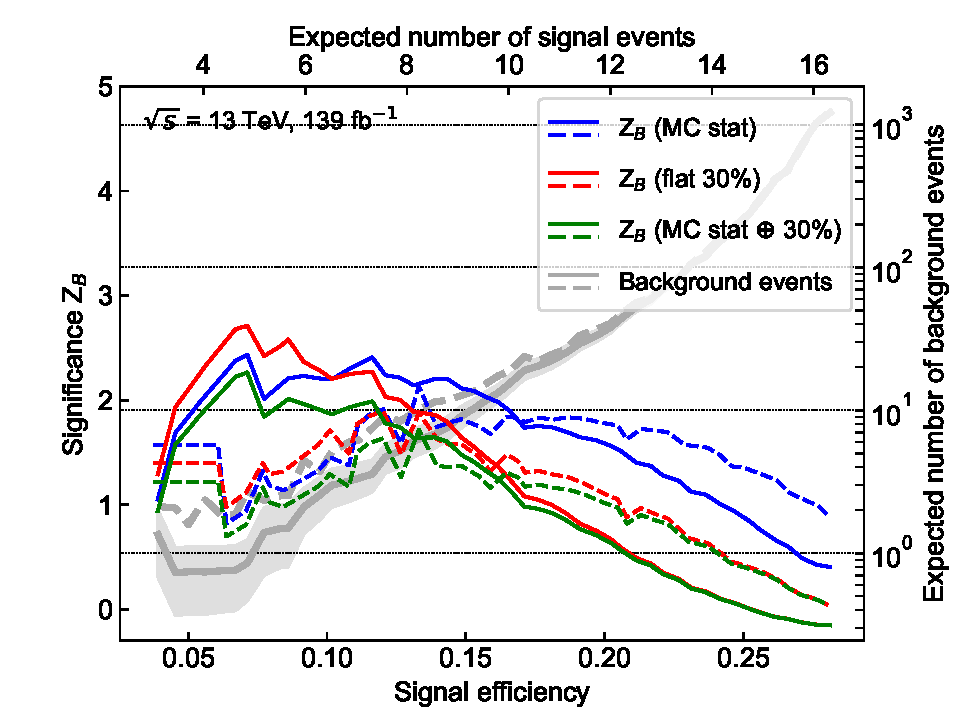
\includegraphics[width=1.0\textwidth]{N-1_cut_scan/z_vs_effs_800_0.pdf}
		\caption{}
	\end{subfigure}\hfill
	\begin{subfigure}[b]{0.5\linewidth}
		\centering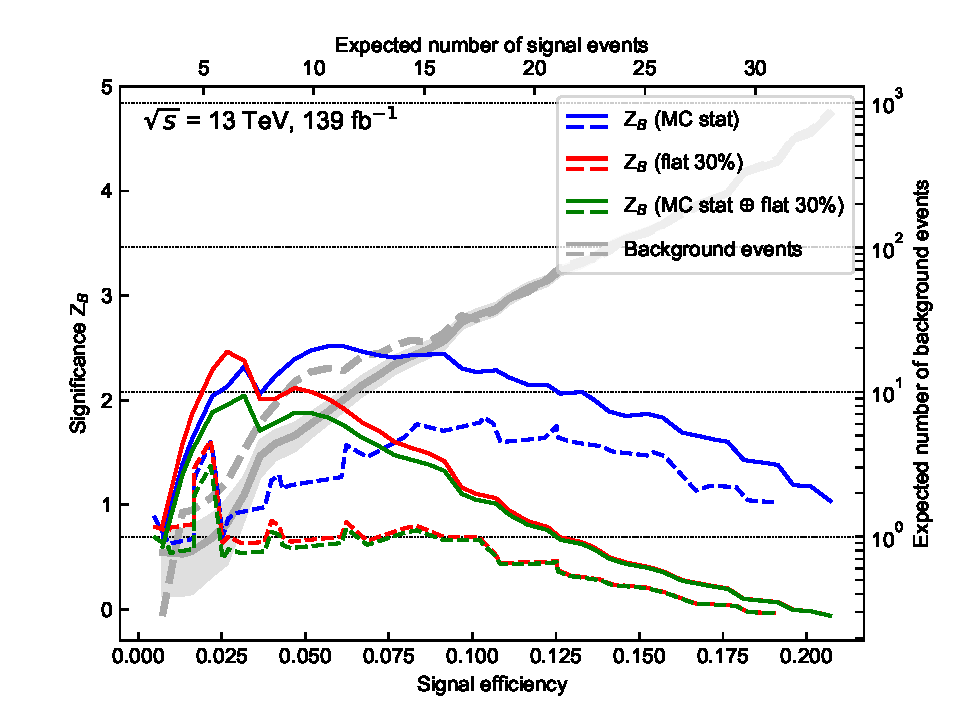
\includegraphics[width=1.0\textwidth]{N-1_cut_scan/z_vs_effs_600_300.pdf}
		\caption{}
	\end{subfigure}\hfill
	\begin{subfigure}[b]{0.5\linewidth}
		\centering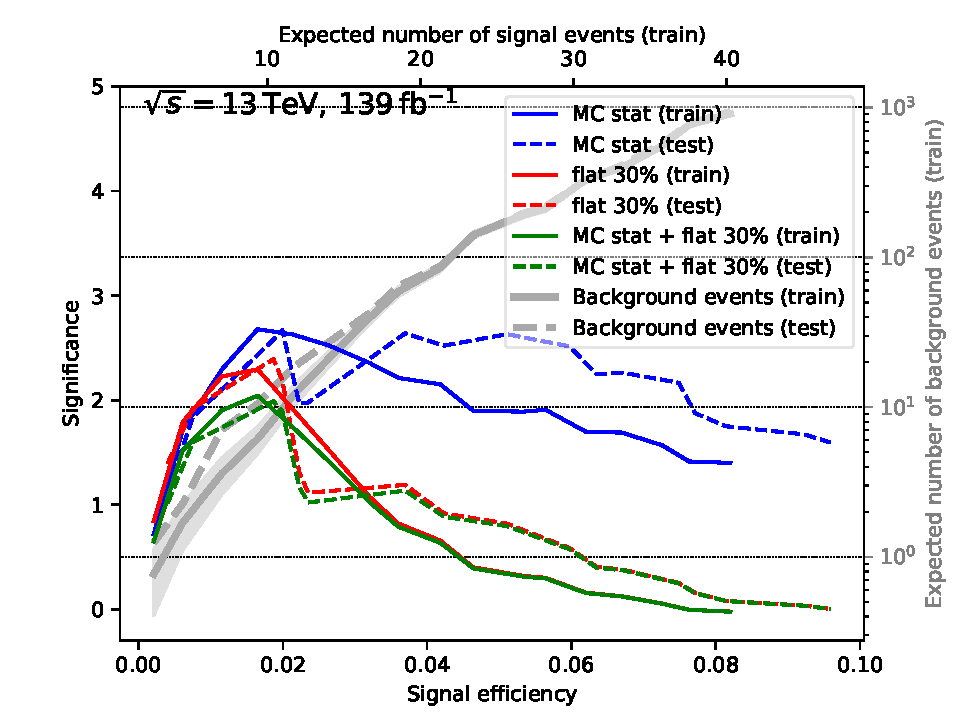
\includegraphics[width=1.0\textwidth]{N-1_cut_scan/z_vs_effs_400_200.pdf}
		\caption{}
	\end{subfigure}\hfill

	\caption[N-dimensional cut scan results]{Results of the $N$-dimensional cut scan for two exemplary benchmark points. The binomial discovery significance $Z_\mathrm{B}$ is plotted against the signal efficiency for varying uncertainty configurations. Additionally, the expected \gls{sm} background rates are shown, including statistical uncertainty for one of the two statistically independent samples (shaded area). The solid and dashed lines represent the two statistically independent subset that the \gls{mc} samples are split into.}
	\label{fig:results_z_vs_eff_rest}
\end{figure}


\begin{figure}
	\centering
	\begin{subfigure}[b]{0.5\linewidth}
		\centering\includegraphics[width=0.7\textwidth]{N-1_cut_scan/n1_800_0/mt}
		\caption{}
	\end{subfigure}\hfill
	\begin{subfigure}[b]{0.5\linewidth}
		\centering\includegraphics[width=0.7\textwidth]{N-1_cut_scan/n1_800_0/mct}
		\caption{}
	\end{subfigure}\hfill
	\begin{subfigure}[b]{0.5\linewidth}
		\centering\includegraphics[width=0.7\textwidth]{N-1_cut_scan/n1_800_0/met}
		\caption{}
	\end{subfigure}\hfill
	\begin{subfigure}[b]{0.5\linewidth}
		\centering\includegraphics[width=0.7\textwidth]{N-1_cut_scan/n1_800_0/mlb1}
		\caption{}
	\end{subfigure}\hfill
	\begin{subfigure}[b]{0.5\linewidth}
		\centering\includegraphics[width=0.7\textwidth]{N-1_cut_scan/n1_800_0/mbb_lower}
		\caption{}
	\end{subfigure}\hfill
	\begin{subfigure}[b]{0.5\linewidth}
		\centering\includegraphics[width=0.7\textwidth]{N-1_cut_scan/n1_800_0/mbb_upper}
		\caption{}
	\end{subfigure}\hfill
	\begin{subfigure}[b]{0.5\linewidth}
		\centering\includegraphics[width=0.7\textwidth]{N-1_cut_scan/n1_800_0/nJet30}
		\caption{}
	\end{subfigure}

	\caption[N-1 plots for the chosen cut combination for the (800, 0) signal point]{N-1 plots for the chosen cut combination for the $(m(\charg/\neutr), m(\lsp)) = (\SI{800}{\GeV}, \SI{0}{\GeV})$ signal point. The shaded region includes \gls{mc} statistical uncertainty as well as 30\% systematic uncertainty (added quadratically) on the background. The significance is computed using the binomial discovery significance using the uncertainty on the background.}
	\label{fig:results_n1_800_0}
\end{figure}



\begin{figure}
	\centering
	\begin{subfigure}[b]{0.5\linewidth}
		\centering\includegraphics[width=0.7\textwidth]{N-1_cut_scan/n1_800_150/mt}
		\caption{}
	\end{subfigure}\hfill
	\begin{subfigure}[b]{0.5\linewidth}
		\centering\includegraphics[width=0.7\textwidth]{N-1_cut_scan/n1_800_150/mct}
		\caption{}
	\end{subfigure}\hfill
	\begin{subfigure}[b]{0.5\linewidth}
		\centering\includegraphics[width=0.7\textwidth]{N-1_cut_scan/n1_800_150/met}
		\caption{}
	\end{subfigure}\hfill
	\begin{subfigure}[b]{0.5\linewidth}
		\centering\includegraphics[width=0.7\textwidth]{N-1_cut_scan/n1_800_150/mlb1}
		\caption{}
	\end{subfigure}\hfill
	\begin{subfigure}[b]{0.5\linewidth}
		\centering\includegraphics[width=0.7\textwidth]{N-1_cut_scan/n1_800_150/mbb_lower}
		\caption{}
	\end{subfigure}\hfill
	\begin{subfigure}[b]{0.5\linewidth}
		\centering\includegraphics[width=0.7\textwidth]{N-1_cut_scan/n1_800_150/mbb_upper}
		\caption{}
	\end{subfigure}\hfill
	\begin{subfigure}[b]{0.5\linewidth}
		\centering\includegraphics[width=0.7\textwidth]{N-1_cut_scan/n1_800_150/nJet30}
		\caption{}
	\end{subfigure}

	\caption[N-1 plots for the chosen cut combination for the (800, 150) signal point]{N-1 plots for the chosen cut combination for the $(m(\charg/\neutr), m(\lsp)) = (\SI{800}{\GeV}, \SI{150}{\GeV})$ signal point. The shaded region includes \gls{mc} statistical uncertainty as well as 30\% systematic uncertainty (added quadratically) on the background. The significance is computed using the binomial discovery significance using the uncertainty on the background.}
	\label{fig:results_n1_800_150}
\end{figure}

\begin{figure}
	\centering
	\begin{subfigure}[b]{0.5\linewidth}
		\centering\includegraphics[width=0.7\textwidth]{N-1_cut_scan/n1_800_250/mt}
		\caption{}
	\end{subfigure}\hfill
	\begin{subfigure}[b]{0.5\linewidth}
		\centering\includegraphics[width=0.7\textwidth]{N-1_cut_scan/n1_800_250/mct}
		\caption{}
	\end{subfigure}\hfill
	\begin{subfigure}[b]{0.5\linewidth}
		\centering\includegraphics[width=0.7\textwidth]{N-1_cut_scan/n1_800_250/met}
		\caption{}
	\end{subfigure}\hfill
	\begin{subfigure}[b]{0.5\linewidth}
		\centering\includegraphics[width=0.7\textwidth]{N-1_cut_scan/n1_800_250/mlb1}
		\caption{}
	\end{subfigure}\hfill
	\begin{subfigure}[b]{0.5\linewidth}
		\centering\includegraphics[width=0.7\textwidth]{N-1_cut_scan/n1_800_250/mbb_lower}
		\caption{}
	\end{subfigure}\hfill
	\begin{subfigure}[b]{0.5\linewidth}
		\centering\includegraphics[width=0.7\textwidth]{N-1_cut_scan/n1_800_250/mbb_upper}
		\caption{}
	\end{subfigure}\hfill
	\begin{subfigure}[b]{0.5\linewidth}
		\centering\includegraphics[width=0.7\textwidth]{N-1_cut_scan/n1_800_250/nJet30}
		\caption{}
	\end{subfigure}

	\caption[N-1 plots for the chosen cut combination for the (800, 250) signal point]{N-1 plots for the chosen cut combination for the $(m(\charg/\neutr), m(\lsp)) = (\SI{800}{\GeV}, \SI{250}{\GeV})$ signal point. The shaded region includes \gls{mc} statistical uncertainty as well as 30\% systematic uncertainty (added quadratically) on the background. The significance is computed using the binomial discovery significance using the uncertainty on the background.}
	\label{fig:results_n1_800_250}
\end{figure}

\begin{figure}
	\centering
	\begin{subfigure}[b]{0.5\linewidth}
		\centering\includegraphics[width=0.7\textwidth]{N-1_cut_scan/n1_600_300/mt}
		\caption{}
	\end{subfigure}\hfill
	\begin{subfigure}[b]{0.5\linewidth}
		\centering\includegraphics[width=0.7\textwidth]{N-1_cut_scan/n1_600_300/mct}
		\caption{}
	\end{subfigure}\hfill
	\begin{subfigure}[b]{0.5\linewidth}
		\centering\includegraphics[width=0.7\textwidth]{N-1_cut_scan/n1_600_300/met}
		\caption{}
	\end{subfigure}\hfill
	\begin{subfigure}[b]{0.5\linewidth}
		\centering\includegraphics[width=0.7\textwidth]{N-1_cut_scan/n1_600_300/mlb1}
		\caption{}
	\end{subfigure}\hfill
	\begin{subfigure}[b]{0.5\linewidth}
		\centering\includegraphics[width=0.7\textwidth]{N-1_cut_scan/n1_600_300/mbb_lower}
		\caption{}
	\end{subfigure}\hfill
	\begin{subfigure}[b]{0.5\linewidth}
		\centering\includegraphics[width=0.7\textwidth]{N-1_cut_scan/n1_600_300/mbb_upper}
		\caption{}
	\end{subfigure}\hfill
	\begin{subfigure}[b]{0.5\linewidth}
		\centering\includegraphics[width=0.7\textwidth]{N-1_cut_scan/n1_600_300/nJet30}
		\caption{}
	\end{subfigure}

	\caption[N-1 plots for the chosen cut combination for the (600, 300) signal point]{N-1 plots for the chosen cut combination for the $(m(\charg/\neutr), m(\lsp)) = (\SI{600}{\GeV}, \SI{300}{\GeV})$ signal point. The shaded region includes \gls{mc} statistical uncertainty as well as 30\% systematic uncertainty (added quadratically) on the background. The significance is computed using the binomial discovery significance using the uncertainty on the background.}
	\label{fig:results_n1_600_300}
\end{figure}

\begin{figure}
	\centering
	\begin{subfigure}[b]{0.5\linewidth}
		\centering\includegraphics[width=0.7\textwidth]{N-1_cut_scan/n1_400_200/mt}
		\caption{}
	\end{subfigure}\hfill
	\begin{subfigure}[b]{0.5\linewidth}
		\centering\includegraphics[width=0.7\textwidth]{N-1_cut_scan/n1_400_200/mct}
		\caption{}
	\end{subfigure}\hfill
	\begin{subfigure}[b]{0.5\linewidth}
		\centering\includegraphics[width=0.7\textwidth]{N-1_cut_scan/n1_400_200/met}
		\caption{}
	\end{subfigure}\hfill
	\begin{subfigure}[b]{0.5\linewidth}
		\centering\includegraphics[width=0.7\textwidth]{N-1_cut_scan/n1_400_200/mlb1}
		\caption{}
	\end{subfigure}\hfill
	\begin{subfigure}[b]{0.5\linewidth}
		\centering\includegraphics[width=0.7\textwidth]{N-1_cut_scan/n1_400_200/mbb_lower}
		\caption{}
	\end{subfigure}\hfill
	\begin{subfigure}[b]{0.5\linewidth}
		\centering\includegraphics[width=0.7\textwidth]{N-1_cut_scan/n1_400_200/mbb_upper}
		\caption{}
	\end{subfigure}\hfill
	\begin{subfigure}[b]{0.5\linewidth}
		\centering\includegraphics[width=0.7\textwidth]{N-1_cut_scan/n1_400_200/nJet30}
		\caption{}
	\end{subfigure}

	\caption[N-1 plots for the chosen cut combination for the (400, 200) signal point]{N-1 plots for the chosen cut combination for the $(m(\charg/\neutr), m(\lsp)) = (\SI{400}{\GeV}, \SI{200}{\GeV})$ signal point. The shaded region includes \gls{mc} statistical uncertainty as well as 30\% systematic uncertainty (added quadratically) on the background. The significance is computed using the binomial discovery significance using the uncertainty on the background.}
	\label{fig:results_n1_400_200}
\end{figure}

\begin{figure}
	\centering
	\begin{subfigure}[b]{0.5\linewidth}
		\centering\includegraphics[width=0.7\textwidth]{N-1_cut_scan/n1_300_150/mt}
		\caption{}
	\end{subfigure}\hfill
	\begin{subfigure}[b]{0.5\linewidth}
		\centering\includegraphics[width=0.7\textwidth]{N-1_cut_scan/n1_300_150/mct}
		\caption{}
	\end{subfigure}\hfill
	\begin{subfigure}[b]{0.5\linewidth}
		\centering\includegraphics[width=0.7\textwidth]{N-1_cut_scan/n1_300_150/met}
		\caption{}
	\end{subfigure}\hfill
	\begin{subfigure}[b]{0.5\linewidth}
		\centering\includegraphics[width=0.7\textwidth]{N-1_cut_scan/n1_300_150/mlb1}
		\caption{}
	\end{subfigure}\hfill
	\begin{subfigure}[b]{0.5\linewidth}
		\centering\includegraphics[width=0.7\textwidth]{N-1_cut_scan/n1_300_150/mbb_lower}
		\caption{}
	\end{subfigure}\hfill
	\begin{subfigure}[b]{0.5\linewidth}
		\centering\includegraphics[width=0.7\textwidth]{N-1_cut_scan/n1_300_150/mbb_upper}
		\caption{}
	\end{subfigure}\hfill
	\begin{subfigure}[b]{0.5\linewidth}
		\centering\includegraphics[width=0.7\textwidth]{N-1_cut_scan/n1_300_150/nJet30}
		\caption{}
	\end{subfigure}

	\caption[N-1 plots for the chosen cut combination for the (300, 150) signal point]{N-1 plots for the chosen cut combination for the $(m(\charg/\neutr), m(\lsp)) = (\SI{300}{\GeV}, \SI{150}{\GeV})$ signal point. The shaded region includes \gls{mc} statistical uncertainty as well as 30\% systematic uncertainty (added quadratically) on the background. The significance is computed using the binomial discovery significance using the uncertainty on the background.}
	\label{fig:results_n1_300_150}
\end{figure}


\begin{figure}
	\centering
	\begin{subfigure}[b]{0.5\linewidth}
		\centering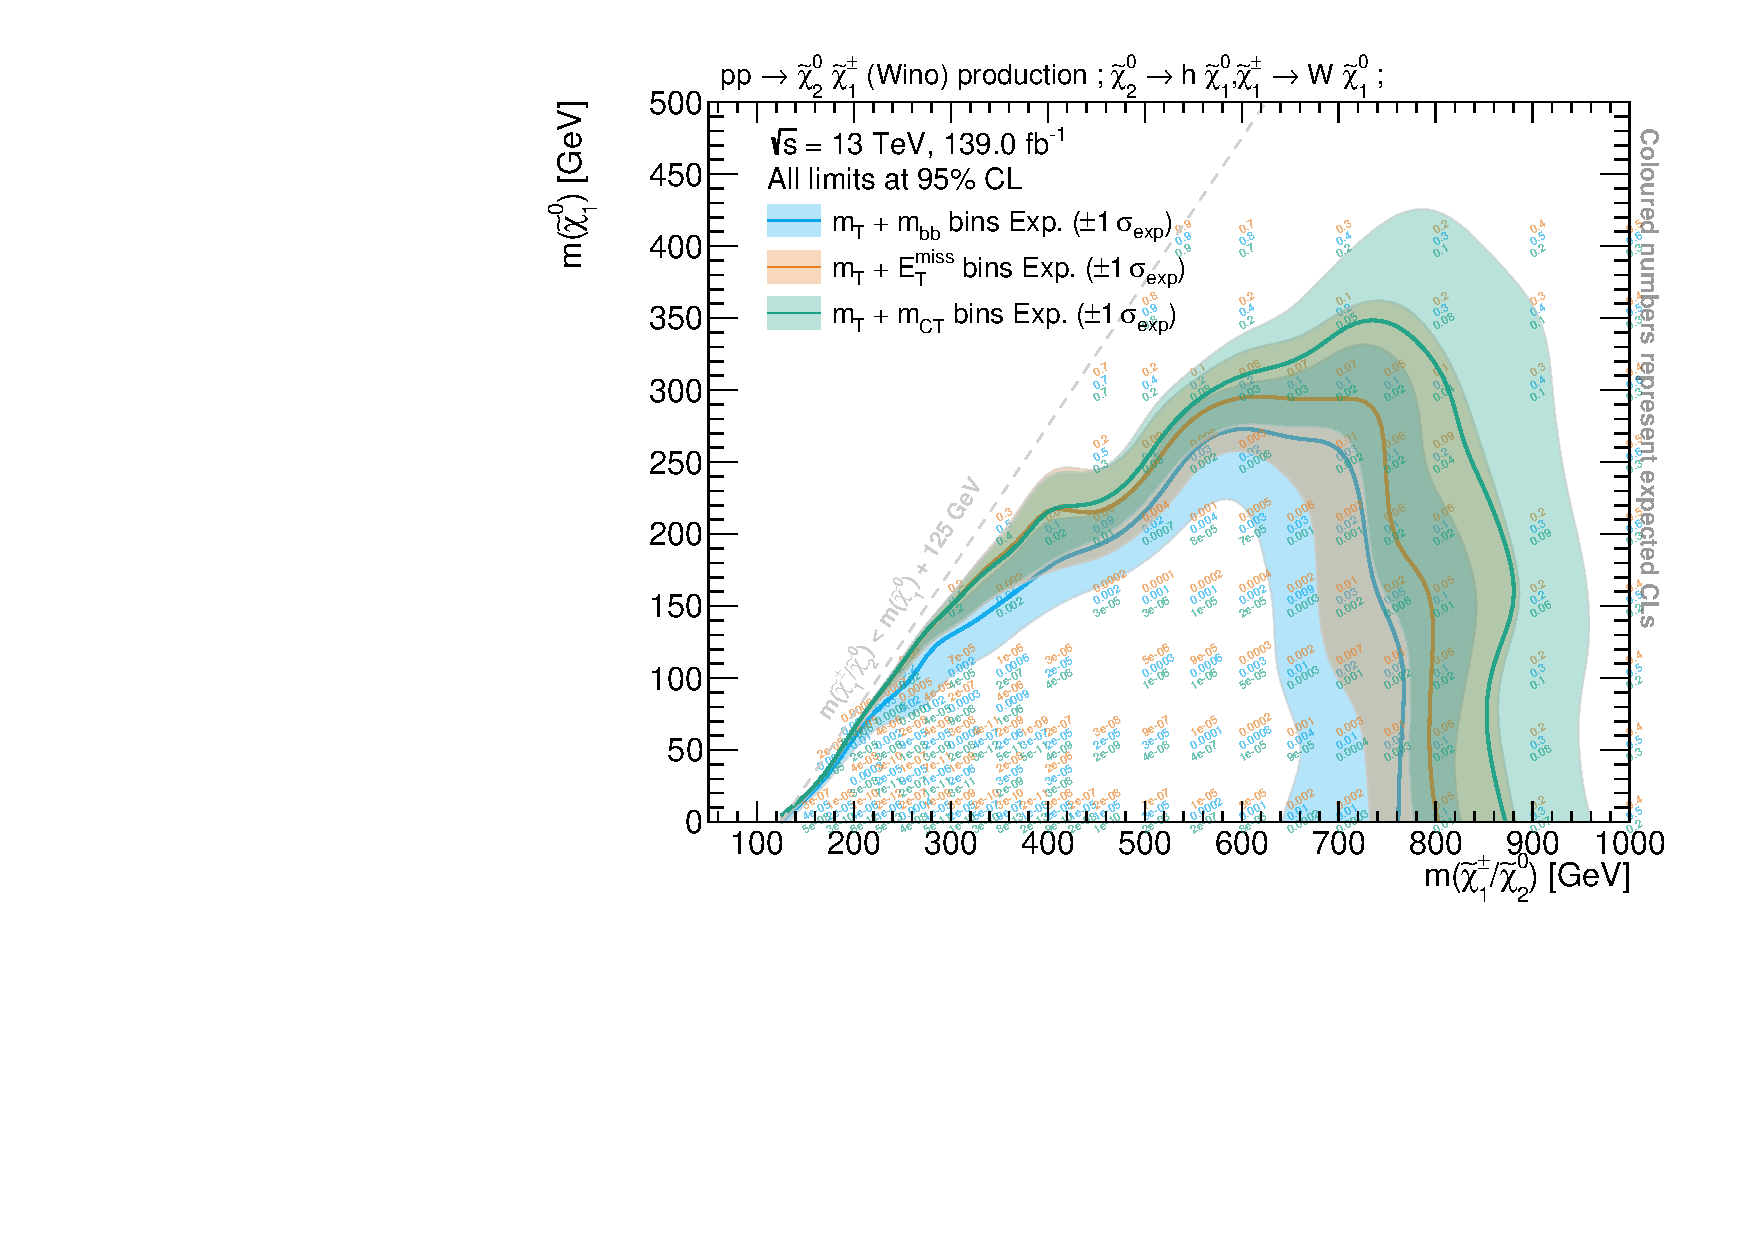
\includegraphics[width=1.0\textwidth]{HF/plot_binnings_cls}
		\caption{\label{fig:plot_binnings_cls}}
	\end{subfigure}\hfill
	\begin{subfigure}[b]{0.5\linewidth}
		\centering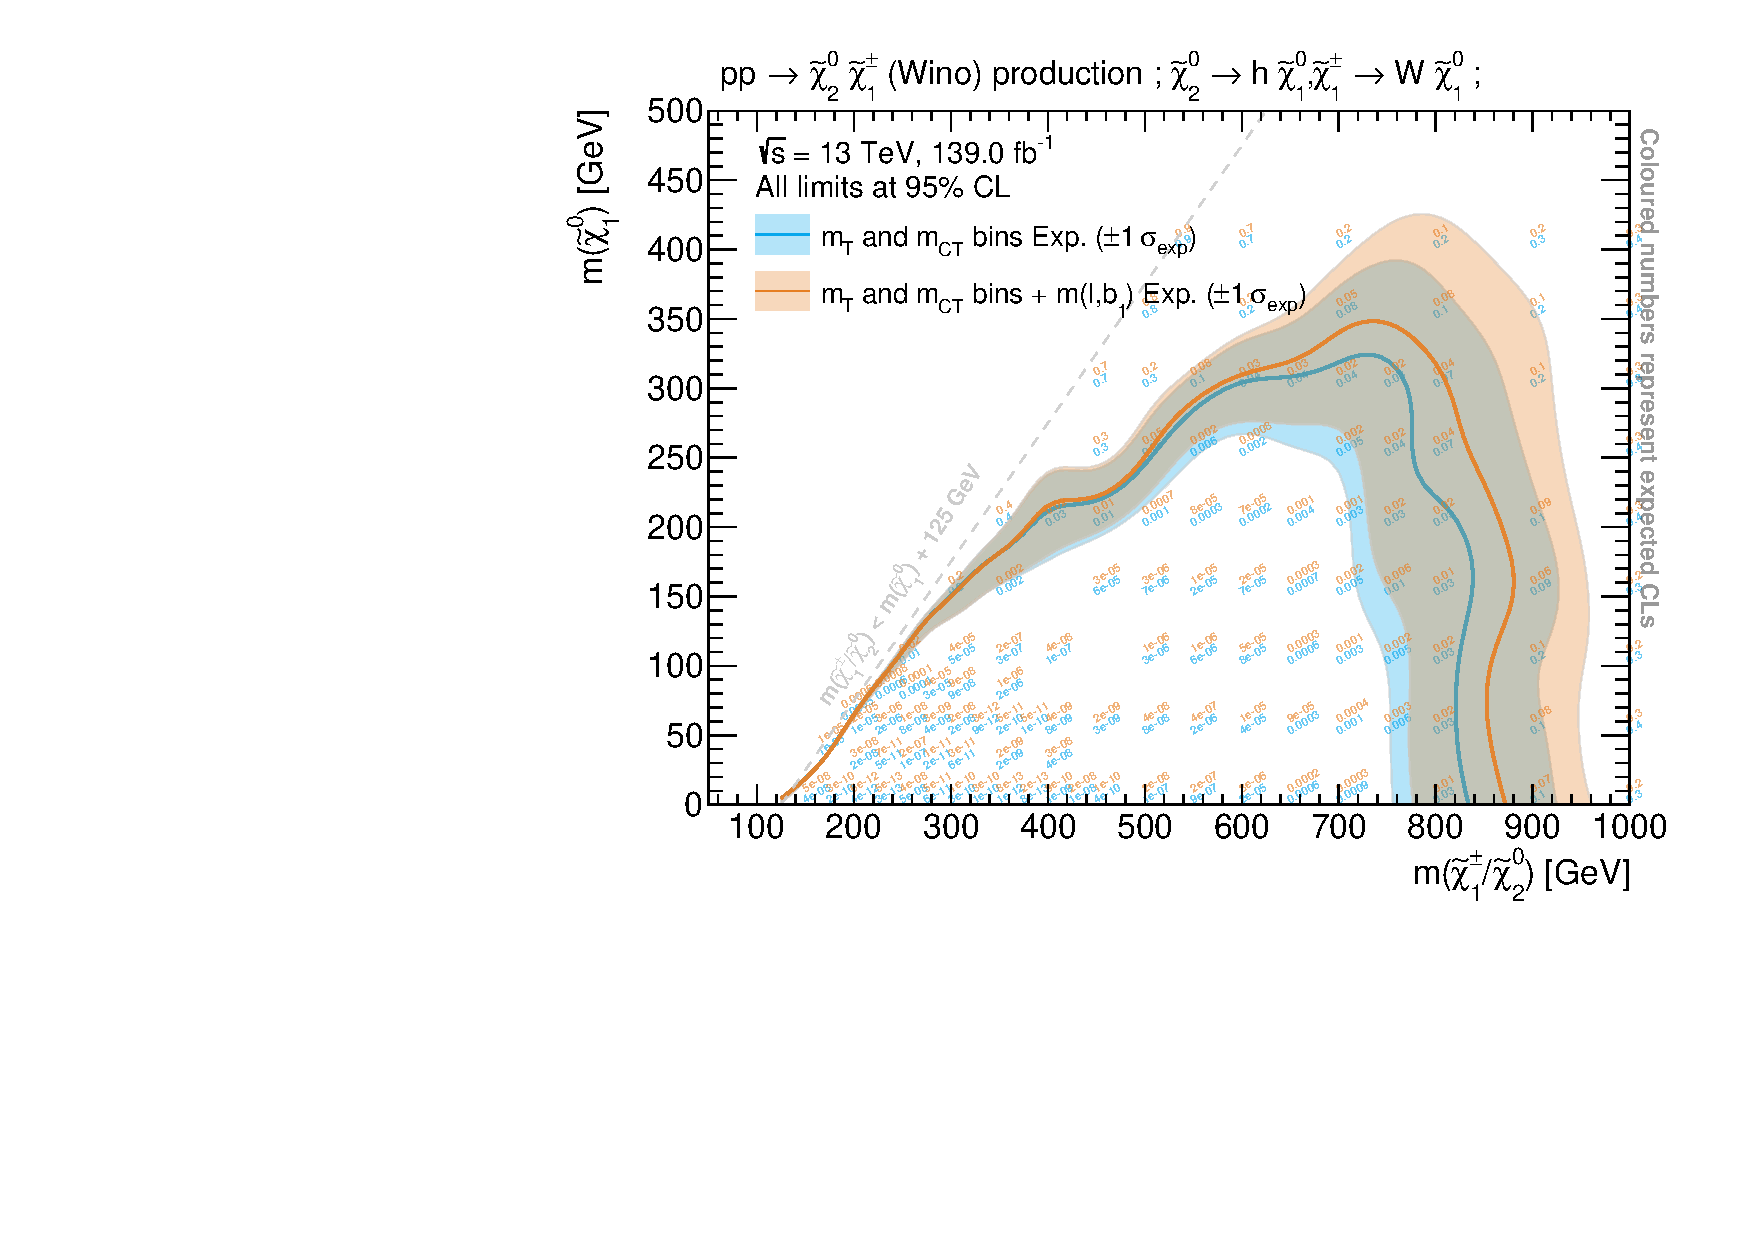
\includegraphics[width=1.0\textwidth]{HF/plot_mlb1_cls}
		\caption{\label{fig:plot_mlb1_cls}}
	\end{subfigure}\hfill
	\begin{subfigure}[b]{0.5\linewidth}
		\centering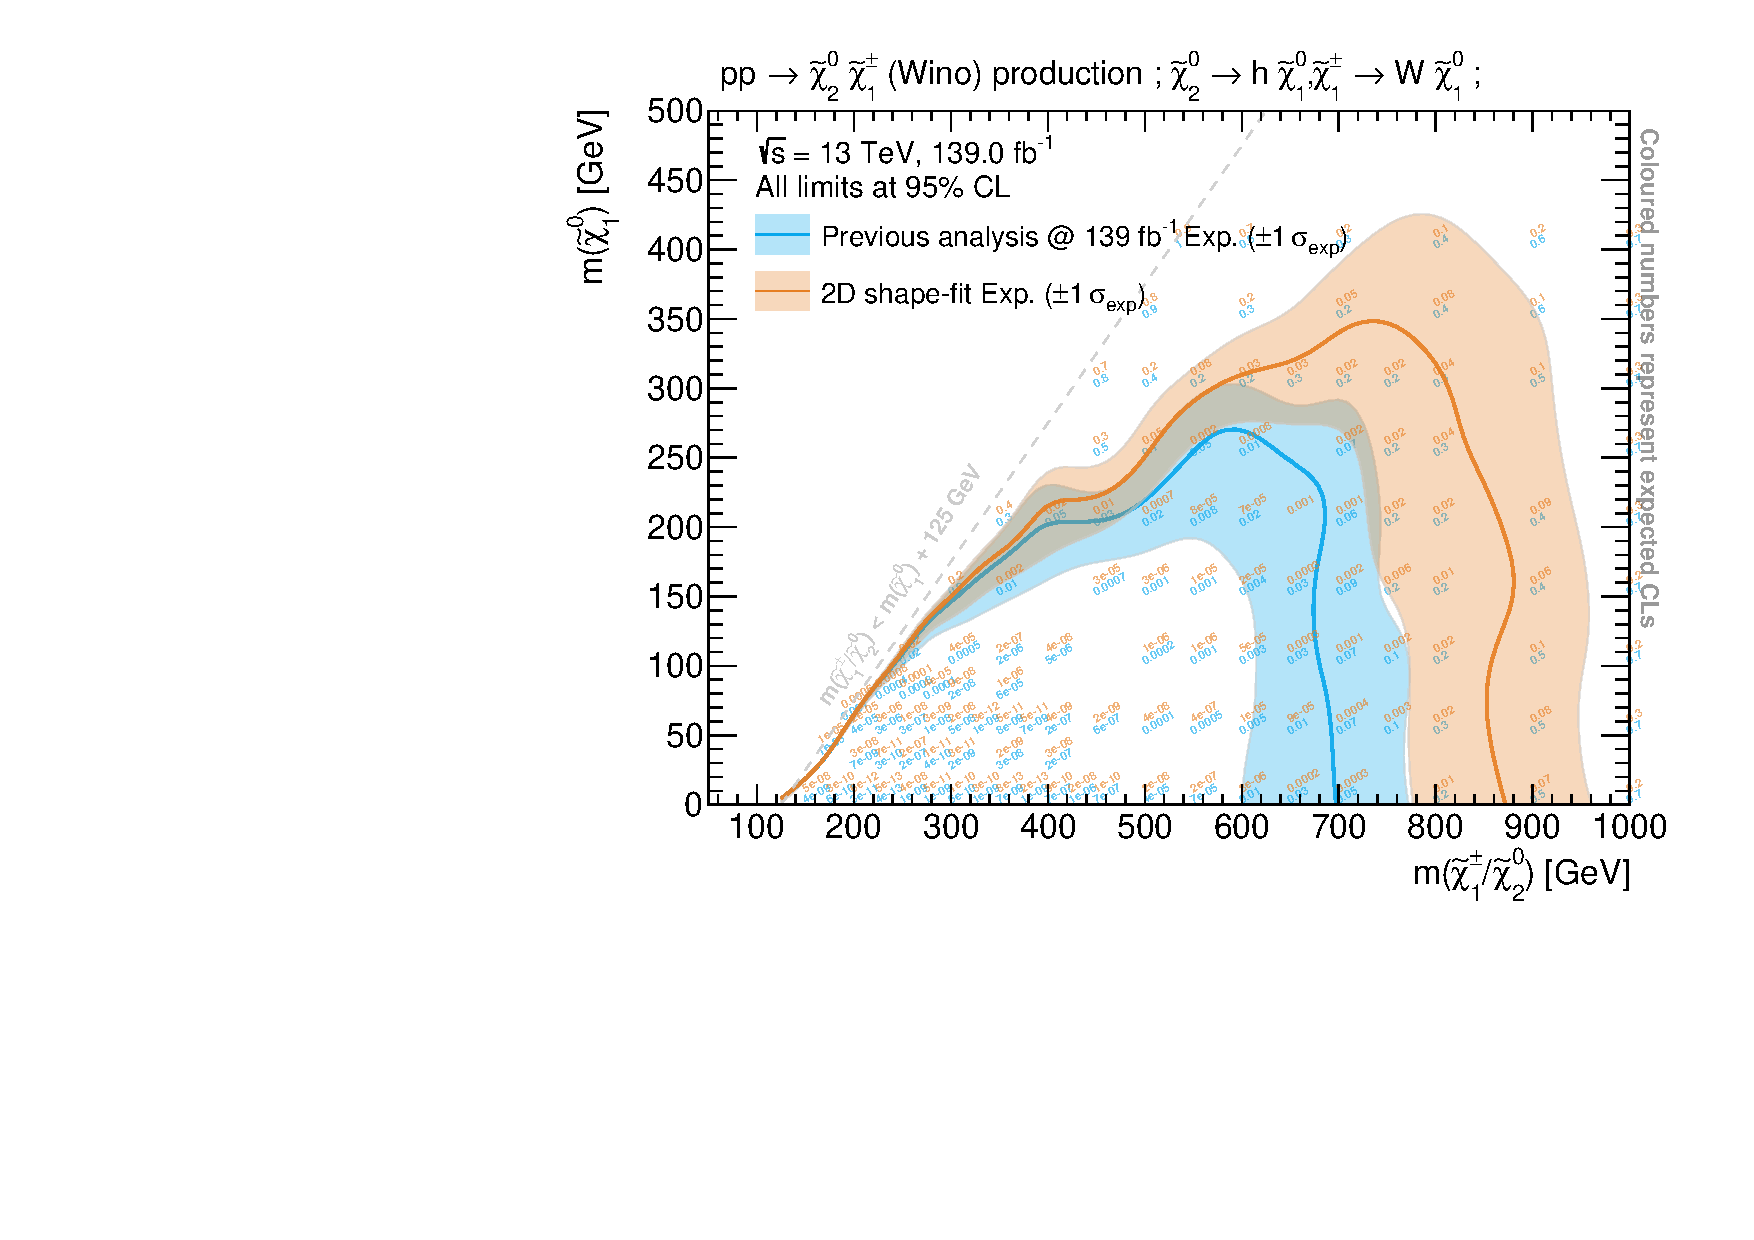
\includegraphics[width=1.0\textwidth]{HF/plot_2d_shapefit_cls}
		\caption{\label{fig:plot_2d_shapefit_cls}}
	\end{subfigure}\hfill

	\caption{}
	\label{fig:results_HF_scan_app}
\end{figure}
